\section{Methodology}
\label{sec:methodology}
We build efficient and accurate SNNs by \textbf{(1)} quantizing SNNs, parametrizing bit widths, and refining the multi-bit spiking neuron formulation out of necessity and  quantization's empiricism; \textbf{(2)} conquering every non-differentiable term and designing  the loss function to achieve controllable bit allocation; \textbf{(3)} formulating the step-size mismatch issue and  alleviating it via the proposed step-size renew.

\subsection{Quantization and parametrization.}
\label{sbsec:quant and param}
\paragraph{Quantization of weight parameters.} 
We first quantize the weight parameters to compress the model size. The quantization formula is as follows:
\begin{align}
w^l_q= clip(\left \lfloor \frac{w_l}{S^l_q} \right \rceil, -2^{B_{w,l}-1}+1, 2^{B_{w,l}-1}-1 )\cdot S^l_q,\label{eq:weight quant}
\end{align}
where  $\lfloor x\rceil$ is the rounding function,  $S_q^l$ represents the learnable quantization step size of layer $l$, $B_{w,l}$ denotes the weight bit width, and $W_q^l$ is the quantized weight value. We further  consider the 1-bit situation, \ie, $B_{w,l}=1$. Then, we would switch  \cref{eq:weight quant} into $w^l_q=sign(w_l/S^l_q)\cdot S^l_q$.
\\\textbf{Parametrization of bit widths.} 
We observe that  \cref{eq:mlif3} is essentially a flooring quantization process of $v^t_l$, where $S_{out,l}^t$ is the quantized integer, $V_{th}$ is the quantization step size, and the quantized spike value is $\alpha \cdot S_{out}^t$. Therefore, SNN's feature map size is controlled by $B_s,T$. Furthermore, the whole model's computation and memory overhead is controlled by $B_s,T,B_w$, which is why the “Bit budget” metric is valid and matters. 

As such, we propose to parametrize these three bit widths to realize controllable and learnable model memory and computation. The parametrization formulas are as follows:
\begin{align}
    B_{s,l} = \left \lfloor clip(\hat{B}_{s,l},1,B_{s,bound})\right \rceil,\label{eq:spike bit param}
\end{align}
where $B_{s,bound}$ is the integer upper bound, which is manually set. $\hat{B}_{s,l}$ is the learnable parameter of $B_{s,l}$. Similarly, 
the parametrization of $T,B_w$ can be obtained:
\begin{align}
    &T_{l} = \left \lfloor clip(\hat{T}_{l},1,T_{bound})\right \rceil,\label{eq:spike len param}\\
    &B_{w,l} = \left \lfloor clip(\hat{B}_{w,l},1,B_{w,bound})\right \rceil.\label{eq:weight bit param}
\end{align}
As the above formulas and notations suggest, we also assign different bit widths to different layers. Consequently, different layer is able to attain suitable bit widths for different data, which makes the allocation of memory and computation adaptive and flexible.
\\\textbf{Formulation of the refined parametric spiking neuron.} 
With the quantization and parametrization implemented, the original multi-bit spiking neuron is not suitable for the following bit width learning process. Therefore, we refine its formulation out of necessity and empiricism.

Firstly, since the temporal length is made parametric and can be totally different among different layers during
training, two issues arise: \textbf{(1)} the gradient requirement, \ie, \emph{$T_{l}$ needs to get involved in the forward pass}; \textbf{(2)} the temporal mismatch between layers. 
For example, the previous layer yields spike train with $T=4$, while the post layer only has 2 temporal bits, \ie, $T=2$. Two time steps of data are wasted. 
To solve these issues, we exploit the temporal flexibility \cite{yao2021temporal}, directly squeezing the spike train through averaging operation as shown in  \cref{eq:our sn1}. Notably, the extra computation brought by squeezing is negligible for it only makes up less than 0.1\% of the total model computation. 

Secondly, the flooring operation in  \cref{eq:mlif3} may induce extra quantization error that incurs model degradation. 
From  value quantization's perspective, it is quite obvious that
flooring operation, compared to the rounding operation, brings in more quantization error. Proof is given in the appendix. Therefore, we offer another choice that a shift can be added to transform  \cref{eq:mlif3} into the rounding operation without changing the spike fire format as in  \cref{eq:our sn3}. For the same reason, we find the time constant $\tau$, apart from increasing stochasticity, is not plausible. So, we should also consider set $\tau=1$. Based on the above insights, we empirically conduct experiments in  \cref{exp:ablation on refined neuron} as support.


Thirdly, the spike amplitude coefficient $\alpha$ is usually defined differently among prior arts  \cite{shen2024conventional, guo2024ternary, xiao2024multi}. Here, we keep consistent with quantization's perspective, and directly unify $V_{th}$ and $\alpha$ as identical, layer-wise, learnable quantization step size as shown in Eq. (\ref{eq:our sn1}-\ref{eq:our sn3}).

Eventually, we formulate our refined multi-bit spiking neuron in the following and illustrate it in  \cref{fig:overview}.
\begin{align}
    &V_{in,l}^t=\sum_j w^{l-1}_q \cdot V^1_{th,l-1}\cdot \frac{1}{T_{l-1}} \sum_t^{T_{l-1}}  S_{l-1}^t,\label{eq:our sn1}\\
&v^t_l=\frac{1}{\tau}v_l^{t-1}+ V^t_{in,l}- S^{t-1}_{out,l}V^1_{th,l},\label{eq:our sn2}
\\
&S^t_{out,l}= clip(\left \lfloor\frac{v^t_l}{V^1_{th, l}}+V^2_{th, l}\right \rfloor, 0, 2^{B_{s,l}}-1 ),\label{eq:our sn3}
\end{align}
where, in our practice, $\tau$ is suggested to 1, $\alpha$ is replaced by the potential threshold $V^1_{th,l}$, and  threshold shift $V^2_{th, l}$ equates to  $0.5sign(v^t_l/V^1_{th,l})$. Beyond this, to further increase the adaptivity \cite{yao2022glif, xing2024spikelm}, we also apply the temporal-wise sharing technique to $V_{th,l}^1$ and $B_{s,l}$, whose details are trivial and deferred to the appendix. Plus, the bidirectional-spike version is provided in the appendix as well. 






\subsection{Learnable bit width} 
\label{sbsec:bit learn}
With parametrized bit widths $B_{s,l}$, $B_{w,l}$ and $T_l$, and learnable quantization step sizes $V^1_{th,l},S^l_q$, we further conquer the non-differentiable terms appearing in the parametrization process, and  constrain bit widths to the target widths. 
\\\textbf{Gradient calculations.} 
We solve non-differentiation via straight-through estimator (STE) \cite{bengio2013estimating} and chain rule. 
% The derivation process is deferred to the appendix. 
\\\textbf{1)} For  $B_{s,l}$, 
\begin{align}
    &\frac{\partial L_{task}}{\partial \hat{B}_{s,l}} = \frac{\partial L_{task}}{\partial B_{s,l}}= \sum^T_t \sum_j \frac{\partial L_{task}}{\partial S^t_{out,l}}  \cdot g_{s,scale}\cdot g_{q}, \\ 
&g_{q} =
\begin{cases}
sign(\frac{v^t_l}{V_{th,l}^1})   \cdot (q_{max}+1),   \cdot    \ln2   , \frac{v^t_l}{V_{th,l}^1}>q_{max} \\0, \text{otherwise}.
\end{cases}
\end{align}
Here, $j$ is the index of the feature map element. The minimum quantization integer $q_{min}=0$ and the maximum integer $q_{max}=2^{B_{s,l}}-1$. While, $g_{s,scale}$, equal to $\frac{1}{\sqrt{\sum_j1\cdot q_{max}}}$ and meant to avoid gradient explosion \cite{esser2020learned}, is the gradient scaling factor. $L_{task}$ represents the task loss signal.
\\\textbf{2)} For  $B_{w,l}$,
\begin{align}
    &\frac{\partial L_{task}}{\partial \hat{B}_{w,l}} = \frac{\partial L_{task}}{\partial B_{w,l}}=  \sum_i \frac{\partial L_{task}}{\partial w^l_q}  \cdot g_{w,scale} \cdot g_{q}, \\ 
&g_{q} =
\begin{cases}
sign( \frac{w_l}{S^l_q})  S^l_q \cdot (q_{max}+1)   \cdot    \ln2   , \frac{w_l}{S^l_q}\notin[q_{min}, q_{max}] \\0, \text{otherwise}.
\end{cases}
\end{align}
Specially, when $B_{w,l}=1$, $q_{min}=-1$ and $q_{max}=1$. Otherwise, $q_{min}=-2^{B_{w,l}-1}+1$ and $q_{max}=2^{B_{w,l}-1}-1$. Similarly,  $i$ is the index of the weight element, and $g_{w,scale} = \frac{1}{\sqrt{\sum_i1\cdot q_{max}}}$.
% \\\textbf{3)} For  $V^1_{th,l}$,
% \begin{align}
% &\frac{\partial L_{task}}{\partial V^1_{th,l}} =  \sum^T_t \sum_j \frac{1}{V^1_{th,l}} \frac{\partial L_{task}}{\partial S^t_{out,l}}  \cdot g_{s,scale}  \cdot g_{q}, \\ 
% &g_{q} =
% \begin{cases}
% \left\lfloor\frac{v^t_l}{V^1_{th,l}}+V_{th,l}^2\right\rfloor - \frac{v^t_l}{V^1_{th,l}}, \frac{v^t_l}{V^1_{th,l}} \in [q_{min},q_{max}]\\
% 0, \frac{v^t_l}{V^1_{th,l}}<q_{min}\\
% q_{max}, q_{max}<\frac{v^t_l}{V^1_{th,l}},
% \end{cases}
% \end{align}
% where all the notations are the same to the case \textbf{1)}.
% \\\textbf{4)} For  $S^l_q$,
% \begin{align}
% &\frac{\partial L_{task}}{\partial S_q^l} =  \sum_i \frac{\partial L_{task}}{\partial w^l_q} \cdot g_{w,scale} \cdot g_{q}, \\ 
% & g_{q}= 
% \begin{cases}
% \left \lfloor \frac{w_l}{S^l_q} \right\rceil - \frac{w_l}{S^l_q}, \frac{w_l}{S^l_q} \in [q_{min}, q_{max}]\text{ and }B_{w,l}>1\\
% sign(\frac{w_l}{S^l_q}) - \frac{w_l}{S^l_q}, \frac{w_l}{S^l_q}\in [q_{min}, q_{max}]\text{ and }B_{w,l}=1\\
% q_{min}, \frac{w_l}{S^l_q}<q_{min}\\
% q_{max}, q_{max}<\frac{w_l}{S^l_q},
% \end{cases}
% \end{align}
% where, notations are all the same to the case \textbf{2)}.
\\\textbf{3)} For $V^1_{th,l}$ and $S^l_q$, the derivation of gradients is similar to prior arts \cite{esser2020learned} and trivial, so we defer it to the appendix.
\\\textbf{4)} For $S^t_{out,l}$ and $T_l$, the only non-differentiable term in the chain rule calculation lies in  \cref{eq:our sn3}, we solve it by STE:
\begin{align}
    \frac{\partial S^t_{out,l}}{\partial (v^t_l/V_{th,l}^1 )} = 
\begin{cases}
1, v^t_l/V_{th,l}^1 \in [q_{min}, q_{max}]\\
0,\text{otherwise}.
\end{cases}
\end{align}
Here, $q_{min}$ and $q_{max}$ are in line with the case \textbf{1)}.
In addition, the gradient calculations for the bidirectional spiking neuron are deferred to the appendix.
\\\textbf{Loss function.} During the supervised training , the bit-width parameters $\hat{B}_{s,l}$, $\hat{B}_{w,l}$, and $\hat{T}_l$ directly obtain the task loss signal $L_{task}$ between the model predictions and labels for optimization, which does not guarantee these bit-width parameters can be compressed towards the target bit widths. Therefore, we proposes a direct constraint on the average bit width of the model in the following:
\begin{equation}
\begin{split}
& L_{total}=L_{task}+\lambda_1L(\bar{B}_w, B^{tar}_w)+\lambda_2L(\bar{T}, T^{tar})\\
&+\lambda_3L(\bar{B}_s, B^{tar}_s), \text{ where } L(x,y)=|| x-y||_2.
\end{split}
\end{equation}
\( B^{tar}_w \), \( T^{tar} \), and \( B^{tar}_s \) represent the target bit widths. \( \lambda_1 \), \( \lambda_2 \), and \( \lambda_3 \) are penalty coefficients. \( \bar{B}_w \) is the average bit width of each weight parameter. \( \bar{T} \) and \( \bar{B}_s \) are feature element's average time step and bit width, respectively.

\subsection{Quantization step size renew}
\label{sbsec:renew}
\paragraph{Quantization step size mismatch issue.} 
Bit width is changeable due to parametrization. If it decreases after the previous parameter update, the current quantization step size in the next forward pass will become unfit because the change of bit width belongs to integer mutation. Consequently, the quantization error would be increased and the model output floats. Here we give a theoretical proof. 

Assuming a variable $x$, \eg, the activation after convolution, submits to $N(0,\sigma^2)$ and is then filtered via ReLU. So, only $x>0$ need be considered because $x=0$ will not incur any quantization error.  We get $x\sim 2N(0,\sigma^2)| x>0$.

\begin{theorem} 
In the quantization process of the variable $x$: $x_q = s\cdot clip(\left\lfloor\frac{x}{s}\right\rceil,0,2^b-1)$, where $x\sim 2N(0,\sigma^2)|  x>0$; $b$ and $s$ respectively denote the bit width and the quantization step size.  
Let the quantization step size $s$ be the statistically optimal: $3\sigma=s\cdot(2^b-1)\Rightarrow s=\frac{3\sigma}{2^b-1}$ and the quantization error $Err=(x-x_q)^2$. If $b$ decreases to $b'$, the quantization error would  
increase by the possibility of $P(x>\frac{2^{b'}-1}{2^{b}-1}\cdot3\sigma| (x\sim 2N(0,\sigma^2),  x>0)) $. 
(Theorem and proof of the bidirectional domain, \ie, no ReLU applied and $x\sim N(0,\sigma^2)$, are in the appendix.)
\end{theorem}
\textbf{Proof 1}\quad
Given $b'<b$ and $x'_q=s\cdot  clip(\left\lfloor\frac{x}{s}\right\rceil,0,2^{b'}-1)$, we obtain $x'_q = x_q - \lambda$, where  $\lambda=s[clip(\left\lfloor\frac{x}{s}\right\rceil,2^{b'}-1,2^b-1)-(2^{b'}-1)]$. Thus, $Err'=(x-x_q+\lambda)^2$. And, the possibility of $P(Err'>Err)$ equates to $P(\lambda > 0)$ (the deduction here is deferred to the appendix). Thus, 
\begin{equation}
\begin{split}
P(\lambda>0) &= P(\frac{x}{s}>2^{b'}-1)\\
&=P(x>\frac{2^{b'}-1}{2^{b}-1}\cdot 3\sigma).
\end{split}
\end{equation}
We conclude that \emph{\textbf{I)} a larger decrease in bit width leads to a higher possibility of increased quantization error.}
\\\textbf{Lemma 1}\quad  Because $b'\le b-1$ and $b'\ge1$, we get $\frac{2^{b'}-1}{2^{b}-1}\le \frac{1}{2}$. Thus, the lower bound of $P(\lambda>0)$ can be calculated:
\begin{equation}
\begin{split}
    P(\lambda>0) > P(x>\frac{3\sigma}{2} ).
\end{split}
\end{equation}
Since $x\sim 2N(0,\sigma^2)$ and $x>0$, we obtain $P(x>\frac{3\sigma}{2} ) = 0.1336>0$. Consider a tensor $X=\{x_1,x_2,...\}^n$, we can conclude that \emph{\textbf{II)}
as bit width decreases, the unchanged step
size would inevitably incur more quantization errors when $X$ has a large dimension $n$.}
% \\\textbf{Lemma 2} Given all the above conditions, we can further calculate the quantization error’s expectation: (the deduction detail is attached in the appendix)
% \begin{equation}
% \begin{split}
%     E(Err') &= s^2[\sum^{2^b-2^{b'}-1}_{j=1} j^2 \cdot P_j \\&+(2^b-2^{b'})^2\cdot P(2^b-\frac{3}{2}<\frac{x}{s})],\\P_j&=P(j+2^{b'}-\frac{3}{2}<\frac{x}{s}<j+s^{b'}-\frac{1}{2}).
%         \label{eq:err expectation}
% \end{split}
% \end{equation}
% Assuming $b$ is fixed, $E(Err')$ would grow as $b'$ declines. Therefore, we conclude that \emph{\textbf{III)} as the amplitude of bit-width decrease increases, so does the likelihood of higher quantization errors.}

With the conclusion \emph{\textbf{I)}} and \emph{\textbf{II)}} combined, 
the step-size mismatch issue can be proven  harmful in direct-training, where bit width mutation constantly occurs between forward passes as shown in  \cref{fig:bit detect}. As the model goes deeper, quantization error would accumulates and further impairs the model output seriously \cite{sengupta2019going}. \emph{The step size mismatch influence could be more severe in SNNs, because the invalid step size will be consecutively used along the temporal dimension in  \cref{eq:mlif3}.} Therefore, the quantization error will also accumulate temporally, causing serious inference offsets. For instance, if $X = \{x_1, x_2,...,x_T\}$, then the possibility of a increased quantization error $(X-X_q)^2$ would be $1-[1-P(x>\frac{2^{b'}-1}{2^b-1}3\sigma)]^T$, which increases as $T$ rises. 
\begin{figure}[t]
  \centering
  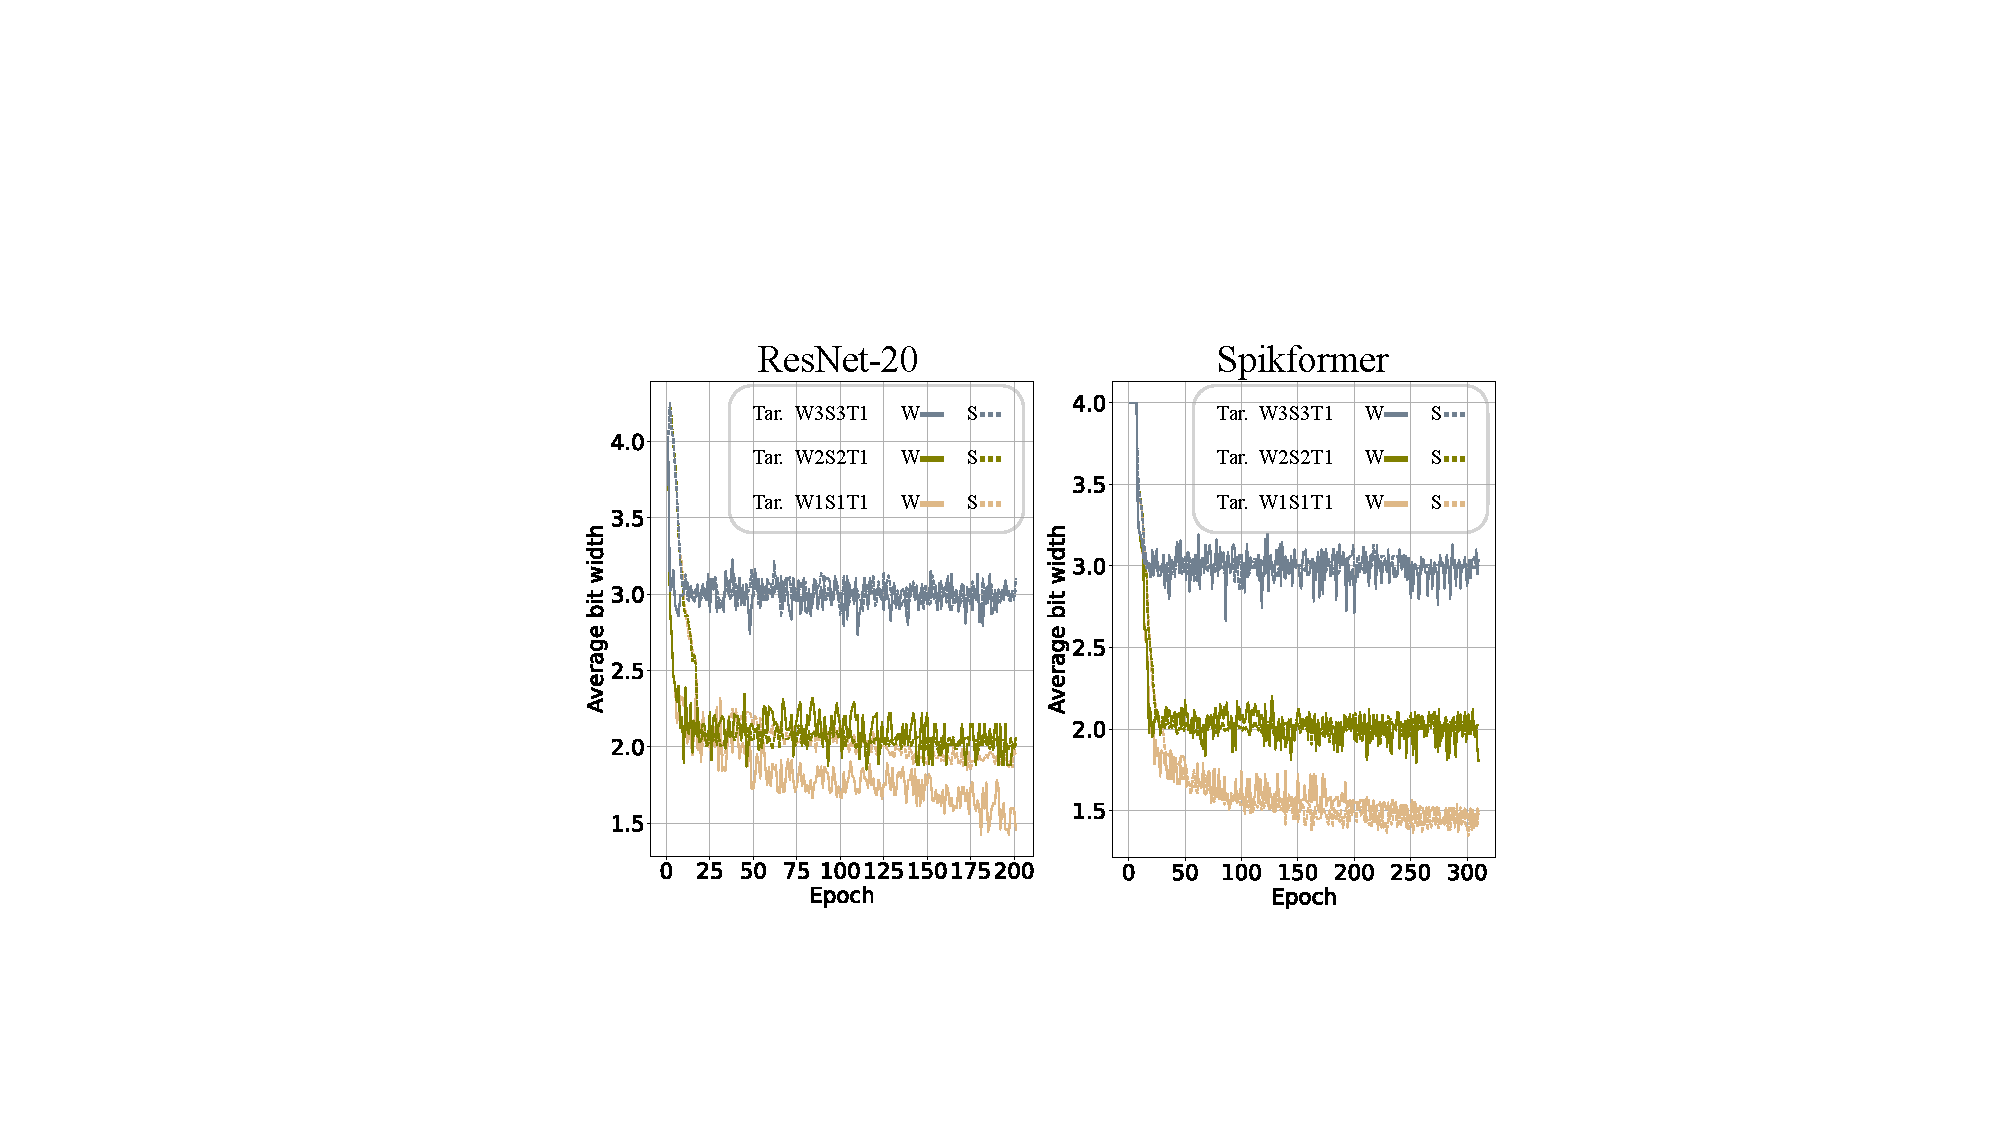
\includegraphics[width= 8cm]{figs/bit detect.pdf}
  \caption{Average bit width changes of ResNet-20 and Spikformer on CIFAR-10 during the adaptive-bit-width training. Tar. abbreviates target bit width. W, S, and T are weight, spike, and temporal bit width, respectively.
  }
  \label{fig:bit detect}
\end{figure}
\\\textbf{Step size renew mechanism.} To alleviate mismatch issue, we propose the following step-size renew mechanism. 
As illustrated in  \cref{fig:overview},
the renew mechanism is based on a bit width observer that watches on the bit width $B_l$, \eg, $B_{w,l}$ and $B_{s,l}$, and records the running maximum $V_{r\_max}$ and minimum $V_{r\_min}$ of the  data to be quantized. $V_{r\_max}$ and $V_{r\_min}$, reflecting the overall data distribution, will be used to renew the step size $S_l$, \eg, $S_q^l$ and $V_{th,l}^1$, directly.


Once $B_l$ is changed, the new $B_l$ will be recorded, the new $q_{max}$ and $q_{max}$ are calculated accordingly, and the observer will also instantly read the current maximum $V_{max}$ and minimum $V_{min}$ of the current batch of data $X$, \eg, weight or activation. 
Based on $V_{max}$ and $V_{min}$, a grid search is performed to calculate the currently optimal maximum $V'_{max}$ and minimum $V'_{min}$  as written in  \cref{algo:grid search}.  Finally, the running maximum $V_{r\_max}$ and minimum $V_{r\_min}$ are updated via 
\begin{equation}
\begin{split}
    &V_{r\_min} = min(V'_{min},V_{r\_min}),\\&V_{r\_max} = max(V'_{max},V_{r\_max}). 
\end{split}
\end{equation}
And, the renewed step size $S_l$ is determined via
\begin{align}
    S_l=\frac{V_{r\_max}-V_{r\_min}}{q_{max}-q_{min}}.
\end{align}

Thus, an optimal $S_l$ can be applied and cover the original one to correct the current forward pass. 
Since the grid search process will consume extra training time, we only activate the renew mechanism in the drastic bit reduction stage. Based on the observations of  \cref{fig:bit detect}, bit reduction mainly occurs in the first 12.5\% epochs. Therefore, we set a shutting threshold that once the difference between the current and the target bit width is below 24\% of the initial difference, the renew mechanism would be deactivated. Consequently, the training time increased by the grid search is lower than 0.05\% of the total training time.

% \begin{figure}[t]
%   \centering
%   \includegraphics[width= 8cm]{figs/reparam_spike_neuron.pdf}
%   \caption{Average bit width changes of ResNet-20 and Spikformer on CIFAR-10 during the adaptive-bit-width training. Tar. abbreviates target bit width, W is weight bit width, and S is the spike bit width.}
%   \label{fig:bit detect}
% \end{figure}


\begin{algorithm}[t]
	% \textsl{}\setstretch{1.8}
	\renewcommand{\algorithmicrequire}{\textbf{Input:}}
	\renewcommand{\algorithmicensure}{\textbf{Output:}}
    \caption{Grid search on $V_{max}$ and $V_{min}$.}
    \label{algo:grid search}
    \begin{algorithmic}[1]
		\REQUIRE Data to be quantized $X$, the $V_{max}$ and $V_{min}$ of $X$, the iteration number $K$, $q_{min}$, $q_{max}$, and the power constant $pow$.
  
		\ENSURE The optimal $V'_{max}$ and $V'_{min}$.

        \STATE $Score\gets 0$, $R\gets V_{max}-V_{min}$, $V'_{max} \gets V_{max}$, and $V'_{min} \gets V_{min}$.

        \STATE for $k=1; k\le K; i++$ do

        \STATE    \quad $V_{max}\gets \frac{k\cdot R}{K} $
        \STATE    \quad if $any(X<0)$ do
        \STATE    \quad \quad $V_{min}\gets -\frac{k\cdot R}{K} $
        \STATE    \quad else do
        \STATE    \quad \quad $V_{min}\gets 0 $
        \STATE  \quad $S'_l\gets\frac{V_{max}-V_{min}}{q_{max}-q_{min}}$ 

        \STATE  \quad $X_{q,k}\gets S'_l\cdot  clip(\left\lfloor\frac{X}{S'_l}\right\rceil,q_{min},q_{max})$
        \STATE  \quad $Score' \gets mean(|X_{q,k}-X|^{pow}) $
        \STATE  \quad if $Score' < Score$ do
        \STATE  \quad \quad $Score\gets Score'$
        \STATE  \quad \quad $V'_{max} \gets V_{max}$ and $V'_{min} \gets V_{min}$
        
    \end{algorithmic}$mean(x)$ is the element-wise averaging function. $any(x)$ checks if at least one element is True.
\end{algorithm}


\begin{table*}[t]
\centering
\caption{Comparisons with existing works on CIFAR. W/S/T denotes the averaged weight/spike/temporal bit width. Our models are initial to W/S/T=4/4/2.}
\label{tab:comparison on cifar}
\begin{adjustbox}{max width=0.9\textwidth}
\begin{threeparttable}
\begin{tabular}{cccccccccc}
\toprule
\multirow{2}{*}{\textbf{Method}} & \multirow{2}{*}{\textbf{Architecture}} & \multicolumn{4}{c}{\textbf{CIFAR 10}}                                                 & \multicolumn{4}{c}{\textbf{CIFAR 100}}                                        \\ \cmidrule(r){3-6} \cmidrule(r){7-10}                                  &                                        & \textbf{W/S/T}       & \textbf{Bit Budget} & \textbf{S-ACE (G)}          & \textbf{Top-1} & \textbf{W/S/T}          & \textbf{Bit Budget} & \textbf{S-ACE (G)}          & \textbf{Top-1} \\ \midrule
\multirow{2}{*}{Dspike \cite{li2021differentiable} }         & \multirow{2}{*}{ResNet20}     & 16/1/2               & 32            & 82.56          & 93.13          & 16/1/2         & 32         & 82.56          & 71.68          \\
                                 &                               & 16/1/4               & 64            & 165.58         & 93.66          & 16/1/4         & 64         & 165.58         & 73.35          \\ 
MLF \cite{fengmulti}                              & ResNet20                      & 16/1/4               & 64            & 165.58         & 94.25          & 16/1/4         & 64         & 165.58         & -              \\ 
\multirow{2}{*}{tdBN \cite{zheng2021going}}           & \multirow{2}{*}{ResNet19}     & 16/1/2               & 32            & 73.28          & 92.34          & 16/1/2         & 32         & 73.28          & -              \\
                                 &                               & 16/1/4               & 64            & 146.56         & 92.92          & 16/1/4         & 64         & 146.56         & -              \\ 
\multirow{2}{*}{TET \cite{deng2021temporal}}           & \multirow{2}{*}{ResNet19}     & 16/1/2               & 32            & 73.28          & 94.16          & 16/1/2         & 32         & 73.28          & 72.87          \\
                                 &                               & 16/1/4               & 64            & 165.12         & 94.44          & 16/1/4         & 64         & 165.12         & 74.47          \\ \midrule
\multirow{3}{*}{Ternary Spike \cite{guo2024ternary}}   & ResNet19                      & 16/2/1               & 32            & 330.24         & 95.58          & 16/2/1         & 32         & 330.24         & 78.45          \\ \cmidrule{2-10} 
                                 & \multirow{2}{*}{ResNet20}     & 16/2/2               & 64            & 165.58         & 94.48          & 16/2/2         & 64         & 165.58         & 73.41          \\
                                 &                               & 16/2/4               & 64            & 330.24         & 94.96          & 16/2/4         & 64         & 330.24         & 74.02          \\ \midrule
\multirow{3}{*}{Multi-bit Spike \cite{xiao2024multi}} & \multirow{3}{*}{ResNet20}     & 16/4/1               & 64            & 165.58         & 94.59          & 16/4/1         & 64         & 165.58         & 75.43          \\
                                 &                               & 16/4/4               & 256           & 660.48         & 94.93          & 16/4/4         & 256        & 660.48         & 76.51          \\
                                 &                               & 16/4/6               & 384           & 990.72         & 95.00          & 16/4/6         & 384        & 990.72         & -              \\ \midrule
\multirow{2}{*}{U-Quant.$\dagger$} & \multirow{2}{*}{ResNet20}     & 4/4/1                & 16            & 41.40          & 96.35          & 4/4/1          & 16         & 41.40          & 79.83          \\
                                 &                               & 4/4/2                & 32            & 82.79          & 96.39          & 4/4/2          & 32         & 82.79          & 80.19          \\ \midrule
Ours-111                         & \multirow{3}{*}{ResNet20}     & \textbf{1.38/1.32/1} & \textbf{1.83}  & \textbf{7.55}           & 96.15          & \textbf{2.06/1.58/3.25} & \textbf{3.25}  & \textbf{13.37}                   & 79.90          \\
Ours-222                         &                               & \textbf{2.13/2/2.08} & \textbf{8.87}  & \textbf{29.75 / 15.93*} & \textbf{96.48} & \textbf{2.11/1.98/2.08} & \textbf{8.66}  & \textbf{32.67 / 18.83*} & \textbf{80.59} \\
Ours-341                         &                               & \textbf{3.01/4.0/1}  & \textbf{12.08} & \textbf{39.49}          & \textbf{97.02} & \textbf{2.88/4.04/1}    & \textbf{11.64} & \textbf{40.60}          & \textbf{81.30}\\ \bottomrule         
\end{tabular}
\begin{tablenotes}
\footnotesize
\item $\dagger$ denotes plain uniform quantization, following  \cite{shen2024conventional}. $*$ denotes the temporal squeezing is applied in inference.  “Ours-xxx” denotes the target bit width of W/S/T.
\end{tablenotes}
\end{threeparttable}
\end{adjustbox}
\end{table*}

\begin{table}[t]
\centering
\caption{Comparisons with existing works on ImageNet.}
\label{tab:comparison on imagenet}
\begin{adjustbox}{max width=0.48\textwidth}
\begin{threeparttable}
\begin{tabular}{cccccc}
\toprule
\textbf{Method} & \textbf{Architecture}         & \textbf{W/S/T}         & \textbf{Bit Budget} & \textbf{S-ACE} & \textbf{Top-1} \\ \midrule
Hybrid training \cite{rathi2020enabling} & ResNet34                      & 16/1/250               & 4000                & 13608          & 61.48          \\
Spiking ResNet \cite{hu2021spiking}  & ResNet50                      & 16/1/350               & 5600                & 18952          & 72.75          \\
tdBN \cite{zheng2021going}           & ResNet34                      & 16/1/6                 & 96                  & 326.60         & 63.72          \\
Dspike \cite{li2021differentiable}         & ResNet34                      & 16/1/6                 & 96                  & 326.60         & 68.19          \\
MS-ResNet \cite{hu2024advancing}       & ResNet34                      & 16/1/6                 & 96                  & 326.60         & 69.42          \\ \midrule
TET \cite{deng2021temporal}             & Sew-ResNet34                  & 16/1/4                 & 64                  & 217.72         & 68.00          \\
Ternary Spike \cite{guo2024ternary}   & ResNet34                      & 16/2/4                 & 128                 & 435.47         & 70.74          \\ 
\multirow{2}{*}{PLIF+SEW \cite{fang2021deep}}     & SEW-ResNet34                  & 16/1/4                 & 64                  & 217.72         & 67.04          \\ 
                & SEW-ResNet50                  & 16/1/4                 & 64                  & 215.62         & 67.78          \\ 
Quant. SNN \cite{shen2024conventional}      & SEW-ResNet34                  & 8/8/1                  & 64                  & 217            & 70.13          \\ \midrule
Ours-221        & \multirow{3}{*}{SEW-ResNet34} & \textbf{2.58/2.18/1.0} & \textbf{5.61}      & \textbf{30.74} & 70.57 \\
Ours-241        &                               & \textbf{2.62/3.96/1.0} & \textbf{10.39}      & \textbf{54.69} & \textbf{72.02} \\
Ours-441        &                               & \textbf{3.93/3.92/1.0} & \textbf{15.4}      & \textbf{77.78} & \textbf{72.82} \\ \bottomrule
\end{tabular}

% \begin{tablenotes}
% \footnotesize
% \item $\dagger$ denotes plain uniform quantization, following  \cite{shen2024conventional}.
% \item $*$ denotes the temporal squeezing is applied in inference.
% \end{tablenotes}
\end{threeparttable}
\end{adjustbox}
\end{table}